% Copy the PDF alongside the manuscript, or adjust the graphics path.
\begin{figure}[t]
  \centering
  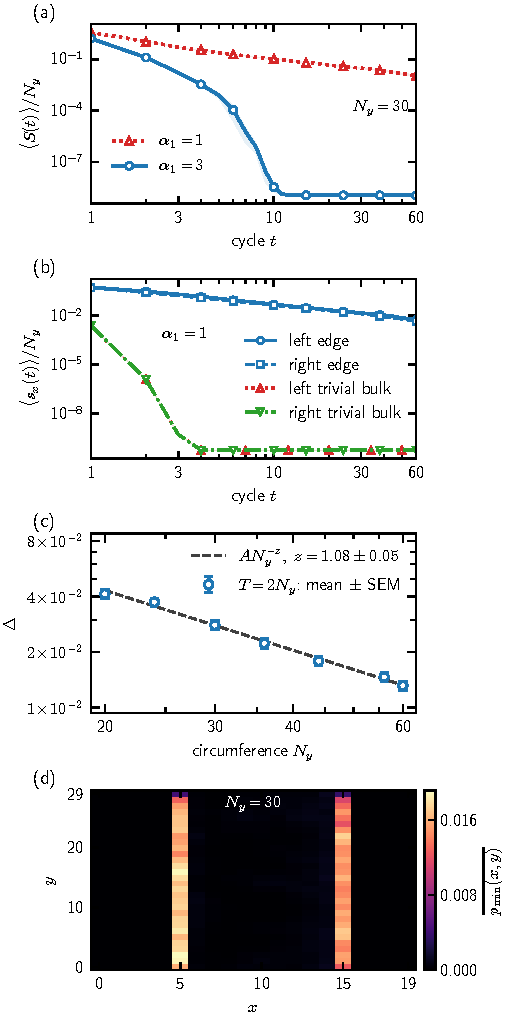
\includegraphics[width=\columnwidth]{purification_ny30_gap_T2Ny_raw_cycles_4x1.pdf}
  \caption{\textbf{Purification and wall-localized slow modes.}
  Hard-wall circuits with $N_x=20$, $n_{\rm shell}=1$, $\alpha_2=30$,
  perfect correction, and raster-$y$ ordering, initialized maximally mixed.
  Panels (a), (b), and (d) use the new full-system-measurement ensembles at
  $N_y=30$, with $100$ independent trajectories per parameter choice and
  final cycle $T=2N_y=60$.
  (a) Mean total entropy per circumference for $\alpha_1=1,3$.
  (b) For $\alpha_1=1$, the entropy contour summed along $y$ at each wall
  ($x=5,15$) and in the trivial slabs ($x=2,18$), divided by $N_y$.
  Panels (a,b) show raw cycle number $t$ on logarithmic axes; cycle zero is omitted from display.
  Shading denotes ordinary trajectory SEM.
  The $\alpha_1=3$ curve retains the original observations through cycle
  $30$ and uses the spectrally clipped continuation thereafter.
  Near-zero entropy tails reflect the occupation cutoff $10^{-12}$ used
  by the entropy estimator.
  (c) On log--log axes, the previously obtained slab-only-measurement size sweep is retained
  separately: trajectory-mean finite-time gaps
  $\Delta=\min_j|\log[(1-\nu_j)/\nu_j]|/(2T)$ at $T=2N_y$,
  with trajectory SEM and an SEM-weighted log-space fit
  $A N_y^{-z}$ over $N_y=20,24,30,36,44,56,60$.
  (d) Mean probability density of the unique minimum-$|\lambda|$ mode,
  selected and normalized separately in each $\alpha_1=1$ trajectory
  at $T=60$, then averaged over trajectories and summed over orbitals.
  Panel (c) is not a size sweep of the new protocol in (a,b,d).}
  \label{fig:purification-restored-scaled-time-gap}
\end{figure}
